%%%%%%%%%%%%%%%%%%%%%%%%%%%%%%%%%%%%%%%%%%%%%%%%%%%%%%%%%%%%%%%%%%%%%%%%%%%%%%%%
%2345678901234567890123456789012345678901234567890123456789012345678901234567890
%        1         2         3         4         5         6         7         8

\documentclass[letterpaper, 10 pt, conference]{ieeeconf}  % Comment this line out if you need a4paper

%\documentclass[a4paper, 10pt, conference]{ieeeconf}      % Use this line for a4 paper

\IEEEoverridecommandlockouts                              % This command is only needed if 
                                                          % you want to use the \thanks command

\overrideIEEEmargins                                      % Needed to meet printer requirements.

%In case you encounter the following error:
%Error 1010 The PDF file may be corrupt (unable to open PDF file) OR
%Error 1000 An error occurred while parsing a contents stream. Unable to analyze the PDF file.
%This is a known problem with pdfLaTeX conversion filter. The file cannot be opened with acrobat reader
%Please use one of the alternatives below to circumvent this error by uncommenting one or the other
%\pdfobjcompresslevel=0
%\pdfminorversion=4

% See the \addtolength command later in the file to balance the column lengths
% on the last page of the document

% The following packages can be found on http:\\www.ctan.org
\usepackage{graphics} % for pdf, bitmapped graphics files
\graphicspath{{figures},}
\usepackage{epsfig} % for postscript graphics files
\usepackage{mathptmx} % assumes new font selection scheme installed
\usepackage{times} % assumes new font selection scheme installed
\usepackage{amsmath} % assumes amsmath package installed
\usepackage{amsfonts}
\usepackage{amssymb}  % assumes amsmath package installed
\usepackage{booktabs} % professional tables (\toprule, \midrule, \cmidrule)
\usepackage{fdsymbol}
\let\proof\relax
\let\endproof\relax
\usepackage{amsthm}
\newtheorem{proposition}{Proposition}
\DeclareMathOperator{\tr}{tr}
\newcommand{\E}{\mathbb{E}}
\newcommand{\cN}{\mathcal{N}}
\DeclareSymbolFont{restoredsy}{OMS}{cmsy}{m}{n} % fdsymbol clobbers \nabla; restore a proper one
\DeclareMathSymbol{\cmnabla}{\mathord}{restoredsy}{"72}
\usepackage{tikz}
\usetikzlibrary{arrows.meta, calc, patterns, angles, quotes, shapes.geometric}

\setlength{\marginparwidth}{2cm}
% \usepackage{todonotes}
\usepackage[disable]{todonotes}
\newcommand{\wouter}[2][] {\todo[inline,backgroundcolor=red!20!white, #1]{(Wouter) #2}} 
\newcommand{\tim}[2][] {\todo[inline,backgroundcolor=green!20!white, #1]{(Tim) #2}} 
\newcommand{\alex}[2][] {\todo[inline,backgroundcolor=purple!20!white, #1]{(Alex) #2}} 
\newcommand{\ajith}[2][] {\todo[inline,backgroundcolor=blue!20!white, #1]{(Ajith) #2}} 


\newcommand\given[1][]{\,#1\vert\,}
\def\-{\text{-}}
\def\+{\text{+}}

\title{\LARGE \bf
% Online Bayesian optimization of central pattern generator parameters in quadrupedal robot locomotion
%Continually learning central pattern generator parameters for quadrupedal robot locomotion with active inference agents
%Event-triggered learning for adaptive central pattern generation\\ in quadrupedal robot locomotion 
%Event-triggered active inference for adaptive central pattern generation in quadrupedal locomotion
%Surprise-triggered re-tuning of central pattern generators for quadrupedal locomotion
%Deciding when and what to re-tune in central pattern generators\\ for quadrupedal locomotion
%Event-triggered active inference for quadrupedal locomotion\\ under payload shifts
Event-triggered active inference for online gait adaptation\\ to sudden payload shifts in quadrupedal locomotion
}


\author{Alex Pitoiset$^{1}$, Tim N. Nisslbeck$^{1}$, Ajith Anil Meera$^{1}$ and Wouter M. Kouw$^{1}$% <-this % stops a space
\thanks{*This work was supported by the Eindhoven Artificial Intelligence Systems Institute and NGF AiNed XS Europe grant.}% <-this % stops a space
\thanks{$^{1}$Department of Electrical Engineering,
        Eindhoven University of Technology, Netherlands
        {\tt\small w.m.kouw@tue.nl}}%
}


\begin{document}



\maketitle
\thispagestyle{empty}
\pagestyle{empty}


%%%%%%%%%%%%%%%%%%%%%%%%%%%%%%%%%%%%%%%%%%%%%%%%%%%%%%%%%%%%%%%%%%%%%%%%%%%%%%%%
\begin{abstract}
Central pattern generators (CPGs) produce efficient rhythmic locomotion from a few parameters, but a set tuned for one operating condition is no longer optimal once that condition changes, even with a reactive attitude controller holding the trunk level.
We augment a coupled-Hopf-oscillator CPG with an attitude virtual model controller and study online re-tuning of its gait parameters.
We separate \emph{when} to change the gait -- a prediction-error trigger that fires when predicted outputs diverge from a goal prior -- from \emph{what} to change it to -- an active inference agent that couples a fast belief over the body's dynamics with a learned map from gait parameters to body outcomes, selecting gaits by minimizing an expected free energy under that prior while remembering which gaits have led to a fall.
Screening each candidate against this memory rather than physically trialing it, as a grid search or Bayesian optimizer must, the agent recovers online without destabilizing trials: on a shifting trunk payload recurring through a continuous bout, it learns within the bout to stop selecting the gaits that fall.
How far this recovery generalizes, and how much the gait parameterization caps it, remain open.
\end{abstract}


%%%%%%%%%%%%%%%%%%%%%%%%%%%%%%%%%%%%%%%%%%%%%%%%%%%%%%%%%%%%%%%%%%%%%%%%%%%%%%%%
\section{INTRODUCTION}

% Efficient locomotion is crucial for animal survival, allowing predator evasion, foraging, and mating. Over millions of years, natural selection has refined both the morphologies and neural control systems of animals, allowing them to navigate in complex and unpredictable conditions with notable efficiency \cite{dickinson2000how}.

Legged machines are increasingly asked to work through long, uninterrupted bouts, across which conditions seldom hold still: the ground changes underfoot, a carried load shifts, an actuator wears down. Each such event can turn a stably walking controller into one that stumbles, so the ability to keep going through it -- an adaptability animals display effortlessly -- separates a laboratory demonstration from a deployable machine. Engineers have long pursued it by replicating animal morphologies \cite{pettersen2017snake, dwivedula2025configbot}, yet the controllers rarely inherit the biological advantage: Boston Dynamics' Spot relies on centralized, sensor-intensive controllers that are effective but complex and costly \cite{dwivedula2025configbot}.

Central pattern generators (CPGs) offer a simpler alternative. In vertebrates, these spinal circuits generate the periodic signals of movements such as walking, freeing higher centers to modulate speed and gait through simple inputs while sensory feedback keeps the rhythm coupled to the body \cite{goulding2009circuits, dickinson2000how}. This decentralized architecture lowers command latency and bandwidth \cite{ijspeert2008special}, making CPG controllers simpler, cheaper, and less energy intensive. The price is that the rhythm is shaped by only a handful of parameters held fixed during walking, and a setting stable under one condition need not be under another; when an event changes the condition mid-bout, staying upright requires re-tuning those parameters online. This paper studies when that re-tuning should be triggered and how the new parameters should be chosen without destabilizing the robot.


%\subsection{Related Work}
Among CPG models, coupled nonlinear oscillators are biologically plausible and computationally efficient \cite{collins1994hard, ijspeert2008special}: mutual inhibition synchronizes the joints into coordinated gaits \cite{collins1994hard, sprowitz2008passive, righetti2008pattern}, and their limit cycles recover quickly from perturbations \cite{sprowitz2008passive} under only a few parameters. An open-loop CPG walks stably on flat ground, but a change in condition induces body rotations the rhythm alone cannot correct, so feedback closes the loop: contact feedback resynchronizes the oscillators to the actual footfalls \cite{righetti2008pattern}, and posture feedback corrects the trunk attitude. Virtual model control (VMC) computes joint actions as if virtual springs and dampers were attached to the body \cite{pratt2001virtual}; Ajallooeian et al.~use such springs to pull the trunk level, traversing terrain that defeats an open-loop CPG \cite{ajallooeian2013central}. We adopt this attitude VMC as a reactive posture layer (Section~\ref{sec:vmc}) and ask a complementary question: given it, when and how should the CPG's gait parameters be re-tuned once the condition changes?

Reactive feedback leaves the parameters untouched; a large or persistent change requires adapting them. Cully et al.~let a damaged robot search a precomputed behavioral repertoire by trial and error, recovering within roughly a dozen physical trials \cite{cully2015robots}, while Kumar et al.~infer a latent encoding of the condition from recent proprioception and adjust a learned policy within a fraction of a second \cite{kumar2021rma}. Each incurs a cost we avoid: trial-and-error executes each candidate on the already-compromised robot, and the learned policy needs extensive training and is opaque. A complementary line instead tunes gait parameters as online black-box optimization: Bayesian optimization fits a Gaussian-process surrogate to the parameter-score pairs seen so far and proposes the next window's parameters, a trust region keeping proposals from jumping to destabilizing gaits \cite{eriksson2019scalable} -- but it too can only score a candidate by walking on it. We instead adapt the few interpretable CPG parameters online and model-based, screening each candidate against a memory of past failures.

We contribute a prediction-error trigger that decides \emph{when} to re-tune the CPG and a unified active inference agent that decides \emph{what} to re-tune to, screening candidates against a memory of failed gaits to avoid the destabilizing on-robot trials that grid search, Bayesian optimization, and extremum-seeking control require. An ablation attributes the reduction in falls to that screening rather than to the unified objective, which matches it while removing the need for a separately tuned detector.

\section{PROBLEM STATEMENT}

We first describe the base platform whose motion defines the locomotion objective, then the controller driving it: a central pattern generator producing the coordinated leg motion, augmented with an attitude virtual model controller that reactively corrects posture.
We then argue that, even with this reactive loop, the parameters yielding stable locomotion depend on the \emph{operating condition} -- the combined state of the environment and the robot's own body -- so a set tuned for one condition degrades once that condition changes, whether externally, as with a different terrain, or intrinsically, as with an added payload or a weakened actuator.
Resuming stable locomotion after such a shift thus requires adapting the parameters online.

\subsection{Base platform and locomotion objective}
\label{sec:base-platform}

%\begin{figure}[htb]
%\centering
%% Schematic side view of the Laikago quadruped, annotated with the CPG's
% actuated joints (hip + knee per leg), walking toward an incline ahead.
% This is a bare tikzpicture fragment: \input it into a document that provides
%   \usepackage{tikz}
%   \usetikzlibrary{arrows.meta, calc, patterns, angles, quotes, shapes.geometric}
% or wrap it in a standalone document to compile to a PDF for \includegraphics.
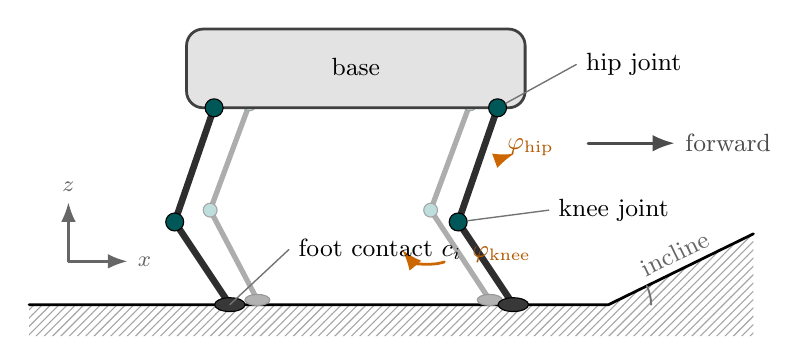
\begin{tikzpicture}[
  >=Latex, line join=round, line cap=round,
  trunk/.style={fill=gray!22, draw=black!75, line width=1pt, rounded corners=6pt},
  link/.style={draw=black!82, line width=2.4pt},
  farlink/.style={draw=black!32, line width=1.9pt},
  joint/.style={circle, fill=teal!68!black, draw=black, inner sep=0pt, minimum size=6.5pt},
  farjoint/.style={circle, fill=teal!25, draw=black!35, inner sep=0pt, minimum size=5pt},
  foot/.style={fill=black!78, draw=black, ellipse, inner sep=0pt,
               minimum width=11pt, minimum height=5pt},
  farfoot/.style={fill=black!30, draw=black!40, ellipse, inner sep=0pt,
                  minimum width=9pt, minimum height=4pt},
  lead/.style={draw=black!55, line width=0.5pt},
  lbl/.style={font=\small},
  ang/.style={draw=orange!80!black, line width=1pt, ->},
]

% ---- ground: flat, then an incline over the front (rightmost) 20% ----
% ground spans x in [-1.4, 7.8] (width 9.2); the ramp runs the last 1.84 (= 20%).
\fill[pattern=north east lines, pattern color=black!35]
  (-1.4,-0.4) -- (-1.4,0) -- (5.96,0) -- (7.8,0.9) -- (7.8,-0.4) -- cycle;
\draw[line width=1pt] (-1.4,0) -- (5.96,0) -- (7.8,0.9);
% small incline-angle marker + label on the ramp
\draw[black!55, line width=0.7pt] (6.5,0) arc (0:26:0.54);
\node[lbl, black!60, rotate=26, anchor=south] at (6.9,0.44) {incline};

% ==== far pair (behind, lighter) ====
% far front
\coordinate (Fh) at (4.2,2.55); \coordinate (Fk) at (3.7,1.2); \coordinate (Ff) at (4.45,0.06);
\draw[farlink] (Fh) -- (Fk) -- (Ff);
\node[farjoint] at (Fh){}; \node[farjoint] at (Fk){}; \node[farfoot] at (Ff){};
% far rear (knee forward, same bend as front)
\coordinate (Rh) at (1.4,2.55); \coordinate (Rk) at (0.9,1.2); \coordinate (Rf) at (1.5,0.06);
\draw[farlink] (Rh) -- (Rk) -- (Rf);
\node[farjoint] at (Rh){}; \node[farjoint] at (Rk){}; \node[farfoot] at (Rf){};

% ==== trunk ====
\draw[trunk] (0.6,2.5) rectangle (4.9,3.5);
\node[lbl] at (2.75,3.02) {base};

% ==== near pair (both knees bend forward, identical geometry) ====
% near front leg
\coordinate (fh) at (4.55,2.5); \coordinate (fk) at (4.05,1.05); \coordinate (ff) at (4.75,0);
\draw[link] (fh) -- (fk) -- (ff);
\node[foot] at (ff){};
% near rear leg
\coordinate (rh) at (0.95,2.5); \coordinate (rk) at (0.45,1.05); \coordinate (rf) at (1.15,0);
\draw[link] (rh) -- (rk) -- (rf);
\node[foot] at (rf){};
\node[joint] (Jfh) at (fh){}; \node[joint] (Jfk) at (fk){};
\node[joint] at (rh){}; \node[joint] at (rk){};

% ==== joint-angle annotations on the near front leg ====
% hip angle: between downward vertical from hip and the thigh
\draw[ang] ($(fh)+(0,-0.62)$) arc (-90:-70:0.62);
\node[lbl, orange!70!black] at ($(fh)+(0.42,-0.5)$) {$\varphi_{\text{hip}}$};
% knee angle: between the thigh extension and the shank
\coordinate (fk_ext) at ($(fk)!-0.7!(fh)$);
\draw[ang] ($(fk)!0.5!(fk_ext)$) arc (-72:-140:0.5);
\node[lbl, orange!70!black] at ($(fk)+(0.55,-0.42)$) {$\varphi_{\text{knee}}$};

% ==== labels with leader lines ====
\draw[lead] (Jfh) -- ($(fh)+(1.0,0.55)$);
\node[lbl, anchor=west] at ($(fh)+(1.0,0.55)$) {hip joint};
\draw[lead] (Jfk) -- ($(fk)+(1.15,0.15)$);
\node[lbl, anchor=west] at ($(fk)+(1.15,0.15)$) {knee joint};
% foot contact, labelled on the near rear foot (belly gap has room)
\draw[lead] (rf) -- ($(rf)+(0.75,0.7)$);
\node[lbl, anchor=west] at ($(rf)+(0.75,0.7)$) {foot contact $c_i$};

% ==== orientation: forward direction + frame ====
\draw[->, line width=1.1pt, black!70] (5.7,2.05) -- (6.8,2.05) node[right, lbl]{forward};
\begin{scope}[shift={(-0.9,0.55)}, black!60, line width=0.9pt]
  \draw[->] (0,0) -- (0.75,0) node[right, font=\footnotesize]{$x$};
  \draw[->] (0,0) -- (0,0.75) node[above, font=\footnotesize]{$z$};
\end{scope}

\end{tikzpicture}

%\caption{The Laikago quadruped, its trunk base state $\xi$, and the twelve leg joints driven by the CPG.}
%\label{fig:laikago}
%\end{figure}

The robot is a floating base actuated through its legs, its trunk described by the base state
\begin{align}
  \xi = (p, \Psi, v, \omega) \,,
  \label{eq:base-state}
\end{align}
collecting the linear position $p \in \mathbb{R}^3$, orientation $\Psi \in SO(3)$, linear velocity $v = \dot{p}$, and angular velocity $\omega$ of the trunk in a world frame.
The orientation is parameterized by roll, pitch, and yaw $(\psi_r, \psi_p, \psi_y)$, of which roll and pitch measure the deviation from upright.

For a given base motion there is a corresponding configuration of the twelve joints, their rates, and the torques that realize it,
\begin{align}
  (\varphi, \dot{\varphi}, \tau) = f(\xi) \,,
  \label{eq:base-to-joints}
\end{align}
where $\varphi$ are the joint angles, $\dot{\varphi}$ their rates, and $\tau$ the torques.
The map $f$ is unknown: it depends on the full rigid-body dynamics, the terrain, and the switching foot--ground contact, none available in closed form.

Locomotion is then the problem of finding torques $\tau$ that drive the base toward a desired behavior: holding a target forward velocity $v^\star$ with roll and pitch near zero,
\begin{align}
  \tau^\star = \arg\min_{\tau} \; \big\lVert v - v^\star \big\rVert + \big\lVert (\psi_r, \psi_p) \big\rVert \,.
  \label{eq:locomotion-objective}
\end{align}
Because $f$ is unknown these torques cannot be solved for directly.
Instead a central pattern generator produces rhythmic joint-angle references, an attitude virtual model controller adjusts them to counter posture deviations, and joint-level position controllers track the result through torques.
We introduce both next.

\subsection{Central Pattern Generator}
\label{sec:cpg}

The CPG is a network of four mutually coupled Hopf oscillators, one per limb -- left front (LF), right front (RF), left hind (LH), right hind (RH) -- coordinated by inhibitory coupling through a gait-specific matrix $K = [k_{ij}]$.
Each oscillator balances stance and swing frequencies through
\begin{equation}
	\omega_i = \omega_{\mathrm{stance}} \varsigma(-b y_i)  + \omega_{\mathrm{swing}} \varsigma(b y_i) \, , \label{eq:omega_i}
\end{equation}
with $\varsigma(\cdot)$ a sigmoid interpolating between the two frequencies by the sign and magnitude of the phase $y_i$, its sharpness set by $b$, and evolves as
\begin{align}
  \dot{x}_i &= \alpha\,(u - r_i^2)\,x_i - \omega_i\,y_i \,, \\
  \dot{y}_i &= \beta\,(u - r_i^2)\,y_i + \omega_i\,x_i
               + \gamma \sum_{j=1}^4 k_{ij}\,y_j + s_i \,, \label{eq:ydot}
\end{align}
where $r_i = \sqrt{x_i^2 + y_i^2}$ is the instantaneous amplitude, $u$ the squared limit-cycle amplitude, and $\alpha, \beta > 0$ convergence rates (typically $\beta \gg \alpha$ for stronger convergence along the $y$-axis).
The coupling gain $\gamma$ strengthens inter-limb coordination and reduces the dependence on initial conditions.

% Different gaits emerge from the choice of the coupling matrix. Figure~\ref{fig:coupling_matrices} illustrates the matrices for trot, pace, bound, and walk, each defining a distinct set of stable phase relationships.
%
The term $s_i$ closes a feedback loop on foot-contact timing \cite{righetti2008pattern}.
Classifying leg $i$ as swinging above a small positive threshold on $y_i$ and in stance below a small negative one (with a hysteresis band between, where $s_i = 0$), and comparing this phase against the binary contact state of foot $i$, yields
\begin{align}
  s_i =
  \begin{cases}
    K_{\text{stop}} \big( \omega_i x_i - \gamma \sum_{j} k_{ij} y_j \big) & \text{contact matches phase} \\
    F_{\text{fast}} \operatorname{sign}(y_i) & \text{otherwise}
  \end{cases}
  \label{eq:feedback}
\end{align}
The phase matches when the foot is airborne in swing or loaded in stance, and is contradicted by an early touchdown or a lost contact; the gains $K_{\text{stop}}$ and $F_{\text{fast}}$ set how strongly the sensed footfalls resynchronize the rhythm to the actual contacts.

The oscillator states map to joint-angle references,
\begin{align}
  \varphi^{\text{hip}}_i &=  \varphi^{\text{hip}}_0  +  A_{\text{hip}}\, x_i , \\
  \varphi^{\text{knee}}_i &= \varphi^{\text{knee}}_0  -  A_{\text{knee}} \max( 0, y_i)  +  \Delta_i ,
  \label{eq:joint-map}
\end{align}
with standing-pose offsets $\varphi^{\text{hip}}_0, \varphi^{\text{knee}}_0$ and swing amplitudes $A_{\text{hip}}, A_{\text{knee}}$: during swing ($y_i > 0$) the knee flexes to lift the foot while the hip advances with $x_i$, and during stance the knee holds its nominal extension.
The term $\Delta_i$ is the posture correction from the virtual model controller of Section~\ref{sec:vmc}, zero for the open-loop CPG.
Joint-level position controllers track these references, producing the torques $\tau$ of Eq.~\ref{eq:base-to-joints}.

The CPG's behavior is governed by a small parameter vector
\begin{align}
    \theta = [\gamma, \omega_{\text{swing}}, \omega_{\text{stance}}, F_{\text{fast}}, K_{\text{stop}}, A_{\text{hip}}, A_{\text{knee}}, b] \,,
    \label{eq:cpg-parameters}
\end{align}
the coupling gain, the stance and swing frequencies, the contact-feedback gains $F_{\text{fast}}$ and $K_{\text{stop}}$, the hip and knee amplitudes, and the sigmoid sharpness $b$.
These set the gait shape and are held fixed during locomotion.

% \begin{figure}[htbp]
%     \centering
%     \includegraphics[width=0.4\textwidth]{Image/Hopf_limitcycle_plot.png}
%     \caption{Limit cycle behavior of Hopf oscillators.}
%     \label{fig:hopf_limit_cycle}
% \end{figure}

\subsection{Attitude Virtual Model Control}
\label{sec:vmc}

The contact feedback of Eq.~\ref{eq:feedback} synchronizes the rhythm to the footfalls, but nothing so far senses the trunk attitude -- yet roll and pitch deviations are precisely what drive the robot toward a fall (Eq.~\ref{eq:locomotion-objective}): on uneven or sloped ground the rhythm induces body rotations it cannot itself correct.
Virtual Model Control (VMC) imagines virtual springs and dampers attached to the robot and computes the joint actions they would produce \cite{pratt2001virtual}.
Ajallooeian et al.~\cite{ajallooeian2013central} span such springs between a trunk-fixed plane and a horizontal reference, so the virtual forces at the stance feet continually pull the trunk level.

We adopt a kinematic form suited to position-controlled joints.
A virtual spring-damper on each attitude angle produces the correction commands
\begin{align}
  c_r &= -\big( \kappa^{r}_{p}\, \psi_r + \kappa^{r}_{d}\, \dot{\psi}_r \big) \,, \label{eq:vmc-roll} \\
  c_p &= -\big( \kappa^{p}_{p}\, (\psi_p - \bar{\psi}_p) + \kappa^{p}_{d}\, \dot{\psi}_p \big) \,, \label{eq:vmc-pitch}
\end{align}
with stiffness and damping gains $\kappa$.
Roll is regulated toward zero, since straight walking involves no sustained bank and lateral tip-over is the dominant fall mode; pitch is regulated toward a slowly adapting baseline $\bar{\psi}_p$ -- an exponential moving average of recent pitch, time constant $\sim\!1$\,s -- so transient rocking is damped while the sustained pitch of an incline is tolerated rather than fought.
The commands distribute over the legs as the knee corrections of Eq.~\ref{eq:joint-map},
\begin{align}
  \Delta_i = \operatorname{clip}\big( \sigma^{F}_i\, c_p + \sigma^{L}_i\, c_r ,\; \pm \delta_{\max} \big) \,,
  \label{eq:vmc-distribution}
\end{align}
with $\sigma^{F}_i = \pm 1$ for front/hind legs, $\sigma^{L}_i = \pm 1$ for left/right legs, and $\delta_{\max}$ bounding the correction.
Since a knee angle sets the effective leg length, the legs on a sinking side of the trunk extend to push that corner up while those on the rising side shorten, realizing the virtual springs of Ajallooeian et al.~\cite{ajallooeian2013central} through the position-controlled knees.

The VMC gains are fixed, hand-tuned, and not part of $\theta$.
The attitude loop thus acts within a stride, correcting momentary deviations but leaving the rhythm itself untouched -- and Ajallooeian et al.~\cite{ajallooeian2013central} observe that these corrections lose effectiveness on harder terrain, where they begin to work against the CPG's forward progression.
Whether locomotion stays stable therefore still hinges on $\theta$ matching the operating condition, which we examine next.

\subsection{Shifts in Parameter Optimality}
\label{sec:optimality-shift}

Let $e$ denote the \emph{operating condition}: the combined state of environment and body the gait must accommodate -- extrinsic factors such as terrain incline, friction, and micro-geometry, together with intrinsic ones such as the trunk's mass distribution and each actuator's torque capacity.
Running the controller with parameters $\theta$ under condition $e$, with the attitude feedback of Section~\ref{sec:vmc} active, induces a distribution $p(\xi \given \theta, e)$ over the base state, which we score by the locomotion objective of Eq.~\ref{eq:locomotion-objective},
\begin{align}
    V(\theta, e) = - \mathbb{E}_{p(\xi \given \theta, e)} \Big[ \frac{1}{v^\star} \big\lVert v - v^\star \big\rVert + \frac{1}{\psi_0} \big\lVert (\psi_r, \psi_p) \big\rVert \Big] \,,
    \label{eq:criterion}
\end{align}
setting $V = -c_f$ on a fall.
The scale $\psi_0$ lets the attitude term dominate, encoding uprightness as the primary requirement; in practice the expectation is a time average over an evaluation window on low-pass-filtered angles, so the gait's rhythmic rocking is not penalized.
The best gait for condition $e$ is the condition-conditioned optimum
\begin{align}
    \theta^{\star}(e) = \underset{\theta}{\arg\max}\; V(\theta, e) \,.
    \label{eq:terrain-optimum}
\end{align}

Crucially, $\theta^{\star}(e)$ is not constant: optimizing Eq.~\ref{eq:criterion} under differing terrain, load, or actuator torque yields distinct parameter vectors, each most stable under the condition it was tuned for, so a change in condition relocates the optimum,
\begin{align}
    \theta^{\star}(e_{\text{old}}) \neq \theta^{\star}(e_{\text{new}}) \,,
    \label{eq:optimality-shift}
\end{align}
a \emph{shift in parameter optimality}.
Such shifts arise externally, as when the robot steps onto a new surface, and intrinsically, as when it picks up a payload or an actuator loses torque, and may drift slowly or jump at a discrete \emph{event}.
The experiments of Section~\ref{sec:experiments} study one abrupt, intrinsic event -- a shifting payload -- that relocates the optimum too sharply for the reactive posture loop alone to absorb.

Because $\theta$ is held fixed, a shift leaves the controller suboptimal and the attitude deviations compound: as the trunk tilts, recovery soon demands more than the bounded feedback of Eq.~\ref{eq:vmc-distribution} can supply, and locomotion fails.
Resuming stable walking therefore requires two decisions -- \emph{when} the optimum has moved, and \emph{what} to re-tune $\theta$ toward -- made online, quickly enough to preserve balance.
The next section addresses both with a single active inference agent, in which one goal prior encoding the objective of Eq.~\ref{eq:locomotion-objective} both detects the shift and selects the new gait.


\section{METHODS}
\label{sec:methods}


\subsection{Unified active inference agent}
\label{sec:agent}

The controller is a single active inference agent organized around one Gaussian \emph{goal prior} over the body outputs $\mathbf{y}_k = (v_x, v_y, \phi, \rho)_k$ --- forward and lateral trunk velocity, pitch and roll --- namely $\bar{p}(\mathbf{y}) = \cN(\mathbf{y}^{\star}, \Sigma^{\star})$ with $\mathbf{y}^{\star} = (v^{\star}, 0, 0, 0)$: walk forward at the target speed, level and straight. Two probabilistic models share this prior.

\emph{A dynamics belief.} A multivariate autoregressive model with exogenous input (MARX) predicts the outputs from their recent past and the measured joint angles $\mathbf{q}_k$,
\begin{align} \label{eq:marx}
    \mathbf{y}_k = \textstyle\sum_{i=1}^{p} A_i\, \mathbf{y}_{k-i} + B\, \mathbf{q}_k + \mathbf{e}_k ,
\end{align}
the exogenous term $B\mathbf{q}_k$ a linear proprioceptive map from joint configuration to body motion. A matrix-normal--Wishart posterior over the coefficients $(A_{1:p}, B)$ and noise precision is updated in closed form at every control step ($100$\,Hz) \cite{meera2026curvature}, giving a Gaussian one-step posterior predictive $\cN(\mu_k, \Sigma_k)$.

\emph{A control map.} A Gaussian process maps the CPG parameters $\theta$ to the outcome outputs, fitted to a persistent memory $\{(\theta_j, \mathbf{y}_j)\}$ of the gaits tried and the outputs they produced (a fall recorded as its degraded output). Only the high-leverage subset of the parameters of Eq.~\ref{eq:cpg-parameters} is searched, the rest held at the incumbent, and the memory persists across recurrences, so the map fills in as the condition repeats and no gait is supplied in advance.

When adaptation is triggered (Section~\ref{sec:trigger}), the agent proposes the gait minimizing the expected free energy of its predicted output under the goal prior,
\begin{align} \label{eq:EFE}
    G(\theta) &= \underbrace{\tfrac{1}{2}(\mu_\theta - \mathbf{y}^{\star})^{\!\top} \Sigma^{\star-1}(\mu_\theta - \mathbf{y}^{\star}) + \tfrac{1}{2}\tr\!\big(\Sigma^{\star-1}\Sigma_\theta\big)}_{\text{goal seeking (cross-entropy to goal)}} \nonumber \\
    & \qquad - \underbrace{\tfrac{1}{2}\ln\!\big|I + \Sigma_\theta \Sigma_n^{-1}\big|}_{\text{information gain}} ,
\end{align}
where $(\mu_\theta, \Sigma_\theta)$ is the GP posterior predictive of the output at $\theta$ and $\Sigma_n$ the observation noise, and it proposes $\hat{\theta} = \arg\min_\theta G(\theta)$ over a quasi-random pool of candidates. Safety is not a separate constraint but a consequence of the goal prior: a gait the memory associates with falling predicts outputs far from $\mathbf{y}^{\star}$, inflating the goal-seeking term, so it is avoided while the agent still explores gaits it has not yet ruled out. The performance of any gait is scored as the log-likelihood of its observed output under $\bar{p}$. Because the agent screens each candidate against its own map before committing, it recovers a gait without the destabilizing on-robot trials a black-box optimizer needs to score a candidate, the property Section~\ref{sec:experiments} turns on.

The two models are coupled rather than stacked: they share one goal prior --- the dynamics belief drives the trigger on the prior's attitude marginal (Section~\ref{sec:trigger}) and the control map proposes the gait under the full prior --- so sensing, triggering and control minimize one free energy.

\subsection{Prediction-error triggering}
\label{sec:trigger}

Re-tuning $\theta$ at every step is wasteful and, as Section~\ref{sec:experiments} shows, actively destabilizing, so the agent adapts only when its own predictions leave the goal. The perturbations the agent must survive threaten the trunk's \emph{uprightness}, not its speed: a shift a slower gait can absorb is tolerable, whereas a tilting trunk is not. The trigger therefore reads the attitude marginal of the goal prior --- the cross-entropy of the dynamics belief's one-step predicted pitch and roll $(\mu_k^{\rho}, \Sigma_k^{\rho})$ to their level target,
\begin{align} \label{eq:trigger-err}
    \epsilon_k &= H\big(\cN(\mu_k^{\rho}, \Sigma_k^{\rho})\,\|\,\bar{p}^{\rho}\big) \\
    &= \tfrac{1}{2}\mu_k^{\rho\top}\Sigma^{\star-1}_{\rho}\mu_k^{\rho} + \tfrac{1}{2}\tr \big(\Sigma^{\star-1}_{\rho}\Sigma_k^{\rho}\big) + c ,
\end{align}
the same cross-entropy-to-goal that Eq.~\ref{eq:EFE} minimizes, restricted to the attitude subspace (the level target has zero mean) and evaluated on the belief rather than a candidate gait: it is small while the trunk is predicted level and grows when a perturbation drives it to tilt, requiring no model of the perturbation and no signal of when it occurs. Standardizing $\epsilon_k$ against a healthy warm-up baseline $(\bar{\epsilon}, s)$ and accumulating the excess in a one-sided CUSUM,
\begin{align} \label{eq:trigger-cusum}
    S_k = \max\big(0,\; S_{k-1} + (\epsilon_k - \bar{\epsilon})/s - \kappa \big) ,
\end{align}
fires an event when $S_k$ exceeds a bound $h$; the slack $\kappa$ is the per-step surprise tolerated as noise. Because the CUSUM integrates over time, it registers the sustained mismatch a perturbation creates while rejecting the stride-frequency ripple that dominates a one-step residual at $100$\,Hz.

The monitor is armed only after a sustained healthy interval past a grace period, so the transient following a recovery is never mistaken for a fresh perturbation. Once a gait is applied the accumulator is reset and held at zero for a settle window covering the ramp-in and one scoring hold, so the ramp transient cannot itself re-trigger; the monitor then latches for the remainder of the event, and a single perturbation therefore draws a single correction. Re-tuning runs only while the trunk is measurably off-level. Reading uprightness alone is what lets the trigger \emph{quiet}: once the robot is upright again it falls silent even under a recovered gait that walks slower or must crab sideways to absorb an asymmetric fault, so the agent stops adapting when it has restored balance rather than chasing a nominal speed it may no longer reach. The forward-velocity preference is not discarded --- it stays in the control objective of Eq.~\ref{eq:EFE}, which keeps seeking speed among the gaits that hold the trunk level. Sensing and control thus read one goal prior two ways: its attitude marginal decides \emph{when} to act, the full prior decides \emph{what} to do.

\subsection{Setting the threshold from the cost of adapting}
\label{sec:threshold}

The bound $h$ in Eq.~\ref{eq:trigger-cusum} need not be tuned, because the accumulator carries units.
Since $\epsilon_k$ is a cross-entropy in nats, $s\,S_k$ is the free energy the agent has forgone, in nats, by holding the incumbent gait since the current excursion began, and $h$ is therefore a \emph{price} rather than a sensitivity.
Adapting carries a price of its own.
Writing $p(\theta) = \cN(\theta_k, \Upsilon^{-1})$ for a prior over gait parameters centered on the gait currently running, whose width states how far the agent expects to have to move, a switch to $\theta_k + \Delta\theta$ costs
\begin{align} \label{eq:switch-cost}
    C(\Delta\theta) = -\ln p(\theta_k + \Delta\theta) + c = \tfrac{1}{2}\Delta\theta^{\top}\Upsilon\,\Delta\theta \,,
\end{align}
paid once at the switch.
The mismatch $\epsilon_k$, by contrast, is a rate, incurred afresh at every step the incumbent is held, so a threshold placed on $\epsilon_k$ itself compares a rate against a one-time cost and cannot be dimensionally consistent.
Such a test is either tripped by transients or, with the cost budget set honestly, silent until the robot is already failing.
Accumulating first removes the inconsistency, and the bound becomes the price,
\begin{align} \label{eq:threshold}
    h = C(\Delta\theta)/s \,,
\end{align}
which turns Eq.~\ref{eq:trigger-cusum} into a payback test: the agent switches at the moment the value given up by not switching has repaid what switching costs, after a delay $h/(\bar{e} - \kappa)$ that shortens as the standardized excess $\bar{e}$ grows.
The slack $\kappa$ retains its usual role of fixing the in-control average run length, now the only quantity calibrated by hand, and the healthy warm-up window supplies the null distribution against which it is set.

Two caveats bound how literally Eq.~\ref{eq:threshold} may be read.
First, $\epsilon_k$ measures the total predicted mismatch, of which only the part lying in the subspace the gait parameters can actually steer is recoverable by adapting; equating $h$ with the switch cost therefore sets a \emph{lower} bound on the principled threshold, and a statistic restricted to that recoverable part, such as the Newton decrement of the goal term under the belief's control gain, would tighten it.
Second, the price is only as meaningful as $\Upsilon$.
At the operating point of Section~\ref{sec:exp-payload} we measure $s = 0.025$\,nats, so the value $h = 5$ used throughout prices a switch at $0.13$\,nats, a move of roughly a fifth of one prior standard deviation, whereas the gaits the agent actually applies lie some twelve standard deviations from the incumbent.
Pricing that realized move under the same prior would delay the trigger to a median of $10.8$\,s after onset and leave it silent altogether in most bouts, long past the fall it exists to prevent.
The discrepancy is informative rather than fatal: the realized move is large because the search explores, not because the correction demands it, so the quantity Eq.~\ref{eq:switch-cost} should price is the correction the belief itself deems necessary, not the exploratory jump the search happens to make.
Deriving $\Delta\theta$ from the belief's control gain, and thereby closing the last hand-set constant, we leave to future work.
The slack is what carries the calibration in the experiments below.
Over the $150$\,s of settled nominal walking the $100$ bouts contain, the standardized excess never exceeds $2.7$, so at $\kappa = 3$ every increment is negative and the accumulator cannot leave zero: no false alarm is possible, whatever $h$ is, and $h$ only imposes a short persistence requirement once a perturbation lifts the excess past the slack.
The transient that follows a recovery is a different matter, reaching several hundred standard deviations and subsiding only after some $15$\,s, and it is the arming logic of Section~\ref{sec:trigger} rather than $\kappa$ that keeps it from firing the trigger.

What the slack buys can be stated precisely.
Writing $e_k = (\epsilon_k - \bar{\epsilon})/s$ for the standardized excess and $T = \inf\{k : S_k > h\}$ for the firing time, the accumulator admits both a deterministic and an exponential guarantee against false alarms.

\begin{proposition} \label{prop:fpr}
Conditional on the warm-up estimates $(\bar{\epsilon}, s)$, the recursion of Eq.~\ref{eq:trigger-cusum} satisfies:
\emph{(i)} if $e_k \leq \kappa$ for every $k \leq n$, then $S_k = 0$ for every $k \leq n$ and $T > n$, for any bound $h > 0$;
\emph{(ii)} if the increments $e_k - \kappa$ are independent and identically distributed with negative mean, and some $\theta^{\star} > 0$ solves $\E\big[e^{\theta^{\star}(e_k - \kappa)}\big] = 1$, then the trigger fires during an unperturbed run of unbounded length with probability at most
\begin{align} \label{eq:lundberg}
    \Pr(T < \infty) \leq e^{-\theta^{\star} h} \,.
\end{align}
\end{proposition}

A proof is given in the Appendix.
Part \emph{(i)} is what governs the experiments: over the $150$\,s of settled nominal walking the observed excess peaks at $2.69$, below $\kappa = 3$, so every increment is negative and no false alarm is possible on that sample regardless of $h$.
Part \emph{(ii)} covers excursions beyond the observed support, and it prices $h$ a second way, as a false-alarm exponent.
For Gaussian $e_k$ with mean $\mu$ and variance $\sigma^2$ the coefficient is available in closed form, $\theta^{\star} = 2(\kappa - \mu)/\sigma^2$, giving $e^{-2\kappa h}$ at the standardized values, or $9 \times 10^{-14}$ here.
That figure is optimistic, because $\epsilon_k$ is strongly autocorrelated at $100$\,Hz (a lag-one correlation of $0.92$, and a long-run variance $8.9$ times the marginal variance on nominal data).
The independence hypothesis can be relaxed to stationarity with geometric mixing, at the cost of a constant in front and with $\theta^{\star}$ the root of the limiting scaled cumulant generating function rather than of the one-step one; substituting the measured long-run variance gives $\theta^{\star} \approx 2.7$ and a false-alarm probability below $10^{-6}$, a weaker but still serviceable exponent.
The remaining hypothesis is the one we can least afford to forget: $(\bar{\epsilon}, s)$ are estimated from a warm-up window of $125$ samples whose integrated autocorrelation time is about $33$, hence roughly four effective samples, so Eq.~\ref{eq:lundberg} is a statement conditional on a scale that is itself imprecise.

No matching bound is claimed in the other direction, and the reason is worth recording.
A false-negative guarantee of the usual kind, bounding the detection delay by $h/(\E_1[e_k] - \kappa)$, requires the post-change increments to have positive mean, whereas the perturbation of Section~\ref{sec:exp-payload} raises the mean standardized excess only to $0.93$ against $\kappa = 3$.
The accumulator therefore still drifts downward after the change and fires through excursions of a heavy-tailed statistic rather than through drift, which is enough in practice, every event in Section~\ref{sec:exp-payload} being detected, but leaves the classical delay bounds inapplicable.
A bound can be recovered by assuming a lower bound $p$ on the conditional probability of an excursion of size $a$ past the slack, whereupon a miss over $M$ blocks has probability at most $(1 - p^{\lceil h/a \rceil})^{M}$, but $p$ is only meaningful conditional on the perturbation remaining uncompensated, which is precisely the quantity the trigger exists to infer.
We therefore treat the false-negative rate as an empirical matter throughout.

\section{EXPERIMENTS}
\label{sec:experiments}

We evaluate the unified active inference agent on the Laikago quadruped in PyBullet, on a perturbation of the robot's own dynamics: a shifting trunk payload (Section~\ref{sec:exp-payload}).
The agent runs with the attitude VMC of Section~\ref{sec:vmc} active and adapts only the high-leverage subset of the parameter vector $\theta$ of Eq.~\ref{eq:cpg-parameters}, within fixed bounds throughout, while adaptation is gated by the prediction-error trigger of Section~\ref{sec:trigger}.
Holding the incumbent gait $\theta^{\star}(\text{flat})$ without adapting is the reference against which the agent is measured.
Control runs at $\Delta t = 0.01$\,s with a target forward velocity of $0.5$\,m/s; each perturbation event is scored by the criterion of Eq.~\ref{eq:criterion} over a hold window with the ramp-in excluded, and gait switches are ramped in over $0.3$\,s so the gait never jumps.

Adaptation runs asynchronously with the simulation, as it would on hardware: the controller steps the physics at $100$\,Hz on one thread while each gait proposal --- the expected-free-energy minimization of Eq.~\ref{eq:EFE}, its Gaussian-process fit included --- is computed concurrently off the control loop, so the simulation never pauses to wait for it.
A proposed gait takes effect only once the computation returns; the optimizer's wall-clock cost therefore appears as a control latency, over which the robot keeps walking on the un-adapted gait, rather than as a frozen clock.
Because each bout is paced to real time, a slower optimizer is charged honestly --- through the extra ground covered before its gait engages --- and we report this compute latency alongside the detection latency below.

\iffalse  % ===== DAMAGE EXPERIMENT COMMENTED OUT (placeholder; to be replaced by a real-robot payload experiment) =====
\subsection{Adapting to actuator damage}
\label{sec:exp-damage}

The first scenario degrades the robot's own actuation.
As the robot walks, one hind leg (the right rear) loses torque: the ceiling on its hip and knee position controllers droops from a healthy $60$\,N\,m to $20$\,N\,m over roughly $1$\,s, a persistent under-actuation of a single leg.
To let the controller compensate this \emph{asymmetric} fault, we split the hip amplitude $A_{\text{hip}}$ of Eq.~\ref{eq:cpg-parameters} into one value per leg, $\{A_{\text{hip}}^{\text{FL}}, A_{\text{hip}}^{\text{FR}}, A_{\text{hip}}^{\text{RL}}, A_{\text{hip}}^{\text{RR}}\}$, and let each method search these four amplitudes.
The incumbent gait $\theta^{\star}(\text{flat})$ holds all four equal --- the symmetric flat-optimal rhythm --- and so cannot express the needed asymmetry, tipping the robot on most occurrences, whereas dropping the weak leg's swing and leaning on the others can keep it upright.
The bout is non-episodic and runs for $300$\,s: the damage persists until the robot falls, after which the leg is healed, the robot stood upright, and the damage recurs $2$ to $8$\,s later.
A controller that never adapts therefore meets the same fault over and over, whereas one that finds a compensating gait simply holds it and walks on.

We compare five arms head to head, each searching the four per-leg hip amplitudes: holding the incumbent (no adaptation); Latin-hypercube sampling (grid search); online Bayesian optimization; a safe Gaussian-process recovery agent (the control map of Section~\ref{sec:agent} with a hand-tuned prediction-error trigger); and a clairvoyant oracle that jumps to a pre-fit compensating gait.
The safe GP agent proposes a gait by minimizing an expected free energy over its Gaussian-process map, and its persistent memory --- seeded only with the fact that the incumbent falls under the damage --- fills in across recurrences within the bout, so it stops reselecting the gaits it has seen fall.
Detection reuses the trigger family of Section~\ref{sec:trigger} in a prediction-error form: a CUSUM on the forward-speed deficit and excess tilt relative to the pre-damage baseline fires when the accumulation crosses a bound, re-armed once the robot has recovered after each heal.

Over one hundred $300$\,s bouts per method, detection averaged $1.34$\,s with no false alarms; the asynchronous gait proposal added a median compute latency of $0.15$\,s for the two Gaussian-process arms (ours and Bayesian optimization), rising to $1.8$\,s in the tail, against under a single control step for the non-learning arms.
Holding the incumbent, the robot falls $25.3 \pm 0.1$ times per bout (mean $\pm$ s.e.m.\ over one hundred seeds), tipping on essentially every recurrence (Fig.~\ref{fig:damage-falls}).
All three online methods roughly halve this --- grid search $11.9 \pm 0.7$ and Bayesian optimization $12.1 \pm 0.5$ falls per bout --- and the safe GP agent is safest at $10.7 \pm 0.5$, its fall accrual flattening as its memory fills (Fig.~\ref{fig:damage-falls}).
Its margin over the black-box optimizers is modest here: under a single weak leg much of the searched space still falls, so a poor candidate is costly to probe on the already-compromised robot rather than merely scoring badly.
A clairvoyant oracle falls only $1.2 \pm 0.05$ times, confirming a compensating gait exists within the per-leg space; and that gait restores near-nominal travel, covering $90$\,m under the fault against the incumbent's $104$\,m of healthy walking (Fig.~\ref{fig:damage-comparison}).
The online adapters, by contrast, reach only a bracing compromise: the gaits they settle on survive but merely limp, holding a reduced forward speed ($V \approx -0.2$) rather than restoring the oracle's near-target walking (Fig.~\ref{fig:damage-timeseries}).
Closing that residual gap --- reaching the fast compensating gait online, without tipping the weakened robot during the search --- is the open problem we revisit in the Discussion.

\begin{figure}[t]
\centering

\includegraphics[width=\columnwidth]{damage_cumulative_falls.pdf}
\caption{Cumulative falls over a $300$\,s continual bout under the weakened right-rear actuator (mean over one hundred seeds). Holding the symmetric incumbent gait accrues falls throughout; the three online methods each roughly halve the count, the safe GP agent lowest and flattening as its memory fills, while a clairvoyant oracle barely falls.}
\label{fig:damage-falls}
\end{figure}

\begin{figure}[t]
\centering

\includegraphics[width=\columnwidth]{damage_method_comparison.pdf}
\caption{Per-method outcome under actuator damage (mean $\pm$ s.e.m., one hundred seeds): falls per bout, root-mean-square body tilt of the surviving gaits, and distance travelled under the fault. The online methods survive at a comparable tilt but cover far less ground than the oracle, which alone restores near-nominal travel.}
\label{fig:damage-comparison}
\end{figure}

\begin{figure}[t]
\centering

\includegraphics[width=\columnwidth]{damage_timeseries_seed0.pdf}
\caption{Forward-speed traces over one bout (shaded where the damage is engaged and the method responding). No adaptation and grid search tip repeatedly; the safe GP agent settles into a steady but reduced-speed gait that it holds for the rest of the bout; the oracle restores near-target speed ($0.5$\,m/s).}
\label{fig:damage-timeseries}
\end{figure}
\fi  % ===== end commented-out damage experiment =====

\begin{figure}[t]
\centering

\includegraphics[width=\columnwidth]{payload_cumulative_falls.pdf}
\caption{Cumulative falls over a $300$\,s continual bout under the persistent payload shift (mean over one hundred seeds). Holding the incumbent gait accrues falls throughout. The three arms that must trial a candidate on the loaded robot (grid search, Bayesian optimization, extremum seeking) each find a tolerant gait early and then largely stop falling, but pay for the search first. The two arms that screen candidates against a memory of past falls, our agent and the safe Gaussian-process ablation, fall far less and are indistinguishable from each other, which locates the benefit in the screening rather than in the unified objective. A clairvoyant oracle never falls.}
\label{fig:payload-falls}
\end{figure}

\begin{figure}[t]
\centering

\includegraphics[width=\columnwidth]{payload_trigger.pdf}
\caption{The uprightness-only trigger over one payload shift (ours). \emph{Top:} forward speed, which the tolerant gait carries slowly backward under the load. \emph{Middle:} the attitude cross-entropy $\epsilon_k$ rests at its healthy baseline and rises when the shift tilts the trunk (shaded orange until the trigger fires, green once the proposed gait is active); it settles above baseline rather than returning to it. \emph{Bottom:} the CUSUM $S_k$ crosses its threshold $h$ within $0.76$\,s, is held at zero through the settle window, and re-crosses later in the bout without drawing a second adaptation, the monitor having latched for the event.}
\label{fig:payload-trigger}
\end{figure}

\subsection{Adapting to payload shifts}
\label{sec:exp-payload}

The second scenario perturbs the robot's mass distribution rather than its actuation.
The Laikago carries an $8$\,kg payload rigidly attached above its trunk, whose own mass is $10$\,kg, and at random intervals the payload shifts off the sagittal plane, $0.215$\,m laterally and $0.20$\,m to the rear, ramped over $1$\,s so the change is a sustained bias rather than an impulse.
The offset then persists: once engaged it is held indefinitely, so the trunk bias compounds until the robot either falls or settles into a gait that tolerates the load.
This offset sits at the edge of recoverability: holding the incumbent gait $\theta^{\star}(\text{flat})$ the robot tips over on $85\%$ of shifts, after a median of $33$\,s under the load, yet a re-tuned gait can stay upright indefinitely, so the perturbation rewards adaptation without being hopeless.
The bout is non-episodic and runs for $300$\,s: whenever the robot falls it is stood upright and the payload recentered, and after $2$ to $8$\,s the shift recurs, so a controller that never adapts meets the same perturbation over and over, whereas one that finds a tolerant gait simply holds it and walks on.
An agent that remembers earlier outcomes should therefore stop repeating the parameter choices that fell.

We evaluate the unified active inference agent of Section~\ref{sec:agent}.
At each detected shift it proposes a gait by minimizing the expected free energy of Eq.~\ref{eq:EFE} over its control map, favoring parameters whose predicted outputs lie near the goal while avoiding the regions its memory associates with falling, and here it searches only the high-leverage subset $\{\gamma, \omega_{\text{swing}}, F_{\text{fast}}, K_{\text{stop}}, b\}$ of Eq.~\ref{eq:cpg-parameters}; the memory persists across recurrences within the trial, so the map fills in as the shift repeats.
Adaptation is triggered by the cross-entropy criterion of Section~\ref{sec:trigger}: the MARX dynamics belief, updated online from the trunk outputs and the measured joint angles, drives the CUSUM once its one-step prediction departs the goal, re-arming once the robot has recovered after each recenter.

Five further arms, each searching that same subset so the comparison is head to head, place the agent among the alternatives.
Three are online optimizers that can judge a candidate gait only by running it: Latin-hypercube sampling (grid search), online Bayesian optimization, and extremum-seeking control, the classical model-free tuner, which dithers each parameter at a distinct frequency and demodulates the event score into a gradient estimate \cite{killingsworth2006extremum}.
Extremum seeking is the sharpest form of the difficulty, since even its exploratory dither must be executed on the already-loaded robot.
The fourth is an ablation that isolates the active inference machinery from safety-filtered search: a Gaussian-process agent that screens candidates against the same memory of past falls, but driven by a hand-tuned prediction-error trigger rather than by the attitude marginal of the goal prior, and carrying no MARX belief of the body's dynamics.
The fifth is a clairvoyant oracle that jumps straight to a pre-fit tolerant gait, an upper anchor on any parameter switch.

Because a tolerant gait, once found, simply keeps walking, we run one hundred $300$\,s bouts per method and report the \emph{cumulative} falls each accrues over a bout rather than a per-event rate (Fig.~\ref{fig:payload-falls}).
Holding the incumbent, the robot falls $5.18 \pm 0.18$ times per bout (mean $\pm$ s.e.m.): it never adapts and tips over on $85\%$ of recurrences.
Our agent instead falls only $0.41 \pm 0.08$ times, finding a tolerant gait after fewer than one fall on average and within the first $20$\,s, after which it holds that gait for the rest of the bout.
The three online optimizers fall in between, at $1.49 \pm 0.08$ (grid search), $1.59 \pm 0.09$ (Bayesian optimization), and $1.94 \pm 0.05$ (extremum seeking) falls per bout, each significantly worse than our agent (Mann-Whitney on per-seed fall counts, $p < 10^{-26}$).
They fall more because each can assess a candidate only by executing it on the already-shifted robot, where a poor candidate tips it over rather than merely scoring badly.
Extremum seeking is worst of the three, significantly worse than both grid search ($p \approx 6 \times 10^{-9}$) and Bayesian optimization ($p \approx 3 \times 10^{-6}$), even though its proposal is the cheapest to compute: its dither is a perturbation applied to the loaded robot by construction, so the exploration it needs to estimate a gradient is paid for in falls.
A clairvoyant oracle never falls, confirming a recoverable gait exists within the searched subset.

The ablation, however, qualifies what the active inference machinery contributes.
The safety-filtered Gaussian-process agent, without the unified trigger and without the MARX belief, falls $0.48 \pm 0.08$ times per bout, statistically indistinguishable from our agent's $0.41 \pm 0.08$ ($p = 0.5$), and its fall accrual tracks ours closely throughout the bout (Fig.~\ref{fig:payload-falls}).
What separates the two groups is therefore whether a candidate is screened against a memory of past falls before it is walked on, not whether the trigger and the controller are read off a single goal prior.
The unified formulation should accordingly be read as an architectural simplification, one objective serving both roles at no cost in falls, rather than as the source of the improvement.
Where it does show a measurable edge is in promptness: the goal-prior trigger detects the shift in $0.93$\,s on average against $1.26$ to $1.38$\,s for the prediction-error monitors driving the other arms, with no false alarms in any arm.
Under the asynchronous protocol the gait proposal costs a median of one control step, as a tolerant gait is usually found before any Gaussian-process fit is needed, rising to $1.74$\,s in the tail once the map is being fit.
The agent also stops re-tuning once a tolerant gait is in place, adapting exactly once per shift event across all one hundred bouts, so it does not chatter (Fig.~\ref{fig:payload-trigger}).
Two measurements qualify what produces that restraint.
The attitude prediction-error does not return to its healthy baseline: it settles about $17\%$ above the pre-shift level, within $10\%$ of baseline on only $5\%$ of bouts, since a load held off-center is never quite free.
The accumulator does re-cross its threshold later in most bouts, and no second adaptation follows because the monitor latches for the remainder of the event.
The restraint is therefore a property of the event logic rather than evidence that the residual mismatch has vanished, and whether re-tuning on that residual would help is untested.

At this offset the tolerant gaits are more compromised than falls alone convey.
Every adapting arm settles into a gait that walks slowly \emph{backward} under the load, at $-0.12$\,m/s for our agent and $-0.14$\,m/s for the three optimizers, against a $0.5$\,m/s forward target.
The clairvoyant oracle is the most retrograde of all at $-0.22$\,m/s, which is the informative part: the pre-fit gait that never falls is itself a backward one, so within this parameter subset no gait both tolerates the offset and makes forward progress.
The benefit here is thus strictly falls avoided, and reaching a gait that walks forward under the load is capped by the gait parameterization, as we discuss next.


\section{DISCUSSION}

Our results separate two aspects of online adaptation that are easily conflated: deciding \emph{when} to change the gait and deciding \emph{what} to change it to.
The prediction-error trigger resolves the first cheaply, firing on a sustained loss of performance rather than on stride-frequency ripple, once per perturbation and not during nominal walking, and it re-arms to catch a recurring sequence.
The second is where the danger lies.
Grid search, Bayesian optimization, and extremum seeking can judge a candidate gait only by walking on it, and on an already-perturbed robot a poor candidate does not merely score badly, it tips the robot over.
Extremum seeking makes the point most sharply: its dither is a deliberate perturbation of the loaded robot, and it is the only method whose gait proposal costs no more than arithmetic, yet it falls more often than the two search methods it is cheaper than.
Our agent instead screens each candidate against a learned map with an explicit memory of past falls, so it avoids these destabilizing trials, and within a single bout its fall rate drops as the memory fills.
It achieves this not by a faster search toward a distant optimum, but by making small, model-guided corrections that avoid the gaits it has seen fail.
This holds even though the CPG is already stabilized by the attitude virtual model controller, so the benefit is complementary to the reactive posture loop rather than a substitute for it.

The ablation locates that benefit precisely, and narrows our claim.
A safety-filtered Gaussian-process agent, given the same fall memory but neither the unified goal-prior trigger nor the dynamics belief, matches our agent's fall rate.
The screening is what pays; unifying detection and control under one objective does not lower the fall count further.
We therefore do not claim the unified formulation as a performance result.
Its argument is economy, one goal prior specifying when to act and what to do, which removes a separately tuned detector and here costs nothing in falls while detecting the shift somewhat sooner.
Whether that economy earns more than parsimony, on perturbations where the detector's threshold is harder to hand-tune than it was here, is untested.

Several limitations qualify these conclusions.
The evaluation is in simulation, over a single intrinsic perturbation and a modest number of recurrences, and the reference optima are computed offline.
More fundamentally, how much adaptation can recover is capped by the gait parameterization itself.
Under this payload offset no gait in the searched subset both tolerates the load and advances: the clairvoyant oracle, which never falls, walks backward at $0.22$\,m/s, and every online method settles somewhere between it and a standstill.
Staying upright and making progress are thus in tension here, and our agent, like the others, resolves it toward staying upright.
That makes the falls comparison a clean one, since all arms pay the same price, but it leaves the more useful question of adapting \emph{without} surrendering the locomotion objective open, and it likely requires a richer parameterization rather than a better search within this one.
A richer control representation, or a model expressive enough to reach the distant optimum without destabilizing exploration, is the central open problem.
Validating on hardware, and across a wider range of perturbations, are natural next steps.

\section{CONCLUSIONS}

We augmented a coupled-Hopf-oscillator CPG with an attitude virtual model controller and studied when and how to re-tune its gait parameters online as the operating condition changes.
A prediction-error trigger decides when to adapt from a sustained loss of performance, and a unified active inference agent decides what to change by selecting parameters from a learned model of the body's response, with a persistent memory of past falls, rather than by physically trialing candidates.
On a shifting trunk payload, the agent learns within a single bout to stop selecting the gaits that fall, recovering without the destabilizing trials that grid search, Bayesian optimization, and extremum seeking require.
An ablation attributes that gain to the memory-screened selection rather than to the unified objective, which matches it on falls while dispensing with a separately tuned detector.
How far this recovery generalizes, and how much the gait parameterization itself caps it, remain open.


%%%%%%%%%%%%%%%%%%%%%%%%%%%%%%%%%%%%%%%%%%%%%%%%%%%%%%%%%%%%%%%%%%%%%%%%%%%%%%%%
\appendix
\section{Proof of Proposition~\ref{prop:fpr}}
\label{appx:fpr}

Write $X_k = e_k - \kappa$ for the increments and $W_n = \sum_{k=1}^{n} X_k$ for their partial sums, with $W_0 = 0$, so that Eq.~\ref{eq:trigger-cusum} reads $S_n = \max(0, S_{n-1} + X_n)$ with $S_0 = 0$.

\emph{(i)} Suppose $e_k \leq \kappa$, that is $X_k \leq 0$, for every $k \leq n$.
The claim $S_k = 0$ follows by induction: it holds at $k = 0$, and if $S_{k-1} = 0$ then $S_k = \max(0, X_k) = 0$.
Since $S_k = 0 \not> h$ for every $k \leq n$ and every $h > 0$, the firing time satisfies $T > n$.
The accumulator thus cannot leave the origin on a stretch whose excess never exceeds the slack, irrespective of how the bound is set.

\emph{(ii)} Unrolling the recursion gives the Lindley representation $S_n = \max_{0 \leq j \leq n}\,(W_n - W_j)$.
The vector $(X_1, \dots, X_n)$ and its reversal $(X_n, \dots, X_1)$ share a distribution, so $S_n$ has, for each $n$, the law of $\max_{0 \leq m \leq n} W_m$, and therefore
\begin{align} \label{eq:lindley}
    \sup_{n \geq 0} S_n \;\overset{d}{=}\; M := \sup_{n \geq 0} W_n \,.
\end{align}
The event $\{T < \infty\}$ is $\{\sup_n S_n > h\}$, whose probability is thus $\Pr(M > h)$.

Let $\theta^{\star} > 0$ satisfy $\E[e^{\theta^{\star} X_k}] = 1$, which exists by hypothesis.
Then $Z_n = \exp(\theta^{\star} W_n)$ is a non-negative martingale with $Z_0 = 1$, since the $X_k$ are independent and identically distributed.
Let $\tau = \inf\{n : W_n > h\}$ and apply the optional stopping theorem at the bounded time $\tau \wedge n$,
\begin{align} \label{eq:stopping}
    1 = \E[Z_{\tau \wedge n}] \geq \E\big[Z_{\tau}\,\mathbf{1}\{\tau \leq n\}\big] \geq e^{\theta^{\star} h}\,\Pr(\tau \leq n) \,,
\end{align}
where the first inequality drops a non-negative contribution and the second uses $W_{\tau} > h$ on $\{\tau \leq n\}$.
Letting $n \to \infty$ and applying monotone convergence to $\Pr(\tau \leq n) \uparrow \Pr(\tau < \infty) = \Pr(M > h)$ yields $\Pr(T < \infty) = \Pr(M > h) \leq e^{-\theta^{\star} h}$, which is Eq.~\ref{eq:lundberg}. \hfill$\blacksquare$

Two consequences are used in Section~\ref{sec:threshold}.
For Gaussian increments with $e_k \sim \cN(\mu, \sigma^2)$ the defining equation reads $\theta(\mu - \kappa) + \theta^2\sigma^2/2 = 0$, whose positive root is $\theta^{\star} = 2(\kappa - \mu)/\sigma^2$, so a standardized statistic gives $\theta^{\star} = 2\kappa$ and a bound $e^{-2\kappa h}$.
When the increments are dependent, the martingale argument applies to the limiting scaled cumulant generating function $\Lambda(\theta) = \lim_{n \to \infty} n^{-1} \ln \E[e^{\theta W_n}]$ in place of the one-step one: for stationary sequences satisfying a geometric mixing condition, $\Lambda$ is finite near the origin and the conclusion becomes $\Pr(T < \infty) \leq C\,e^{-\theta^{\star} h}$ with $\Lambda(\theta^{\star}) = 0$ and a constant $C \geq 1$ set by the mixing rate.
The exponent then degrades roughly in proportion to the ratio of long-run to marginal variance, which is the substitution reported in Section~\ref{sec:threshold}.
Both statements are conditional on the warm-up estimates $(\bar{\epsilon}, s)$ that define $e_k$.

%%%%%%%%%%%%%%%%%%%%%%%%%%%%%%%%%%%%%%%%%%%%%%%%%%%%%%%%%%%%%%%%%%%%%%%%%%%%%%%%

\bibliography{references}
\bibliographystyle{plain}

\end{document}
